\begin{frame}[plain]
    \begin{center}
        {\LARGE\bfseries \hollowtext{RAIN}, and how I learned to love it\par}
        \vspace{4mm}
        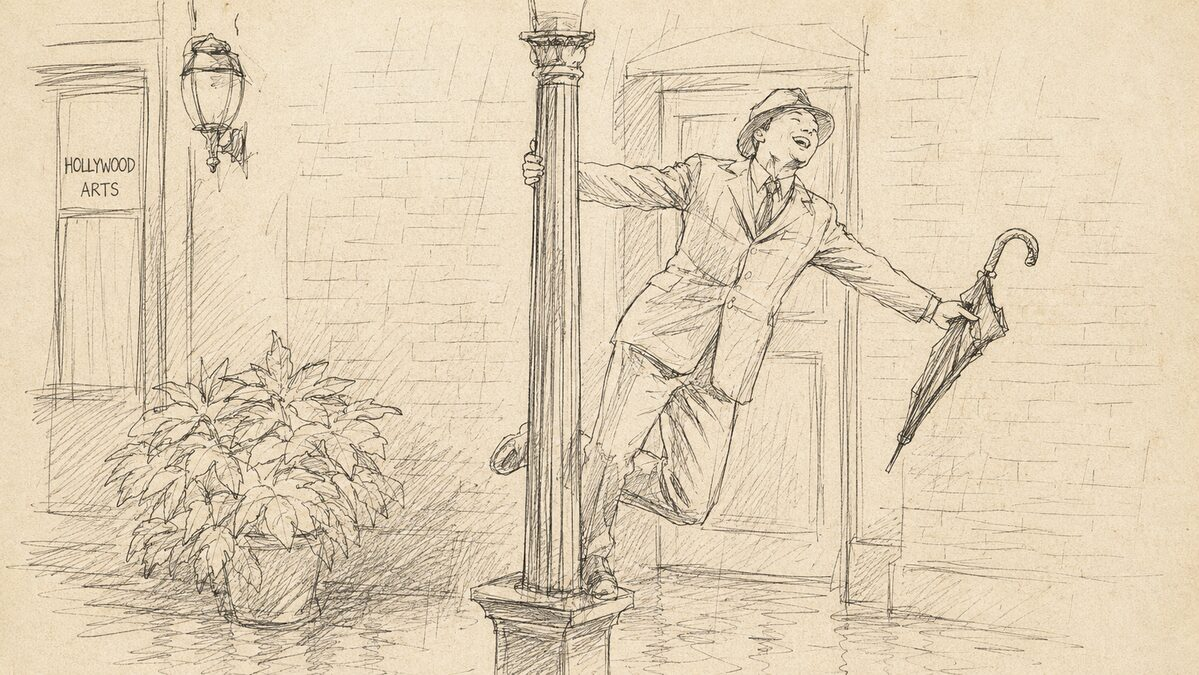
\includegraphics[width=0.92\textwidth,height=0.76\textheight,keepaspectratio]{sing.jpg}
    \end{center}
\end{frame}

%%%%%%%%%%%%%%%%%%%%%%%%%%%%%%%%%%%%%%%%%%%%%%%%%%

\begin{frame}[plain]
    \vspace{-0.5mm}
    \begin{center}
        \large\bfseries welcome to the world of
        
\begin{tikzpicture}[baseline=(ain.base)]
            \node[inner sep=0pt, outer sep=0pt, anchor=base east] (p) at (0,0) {P};
            \draw[red, line width=1.1pt] (p.south west) -- (p.north east);
            \node[red, inner sep=0pt, outer sep=0pt, yshift=0.65ex] at (p.center) {R};
            \node[inner sep=0pt, outer sep=0pt, anchor=base west] (ain) at (0,0) {AIN};
        \end{tikzpicture}
    \end{center}
    \vspace{1mm}

    \centering
    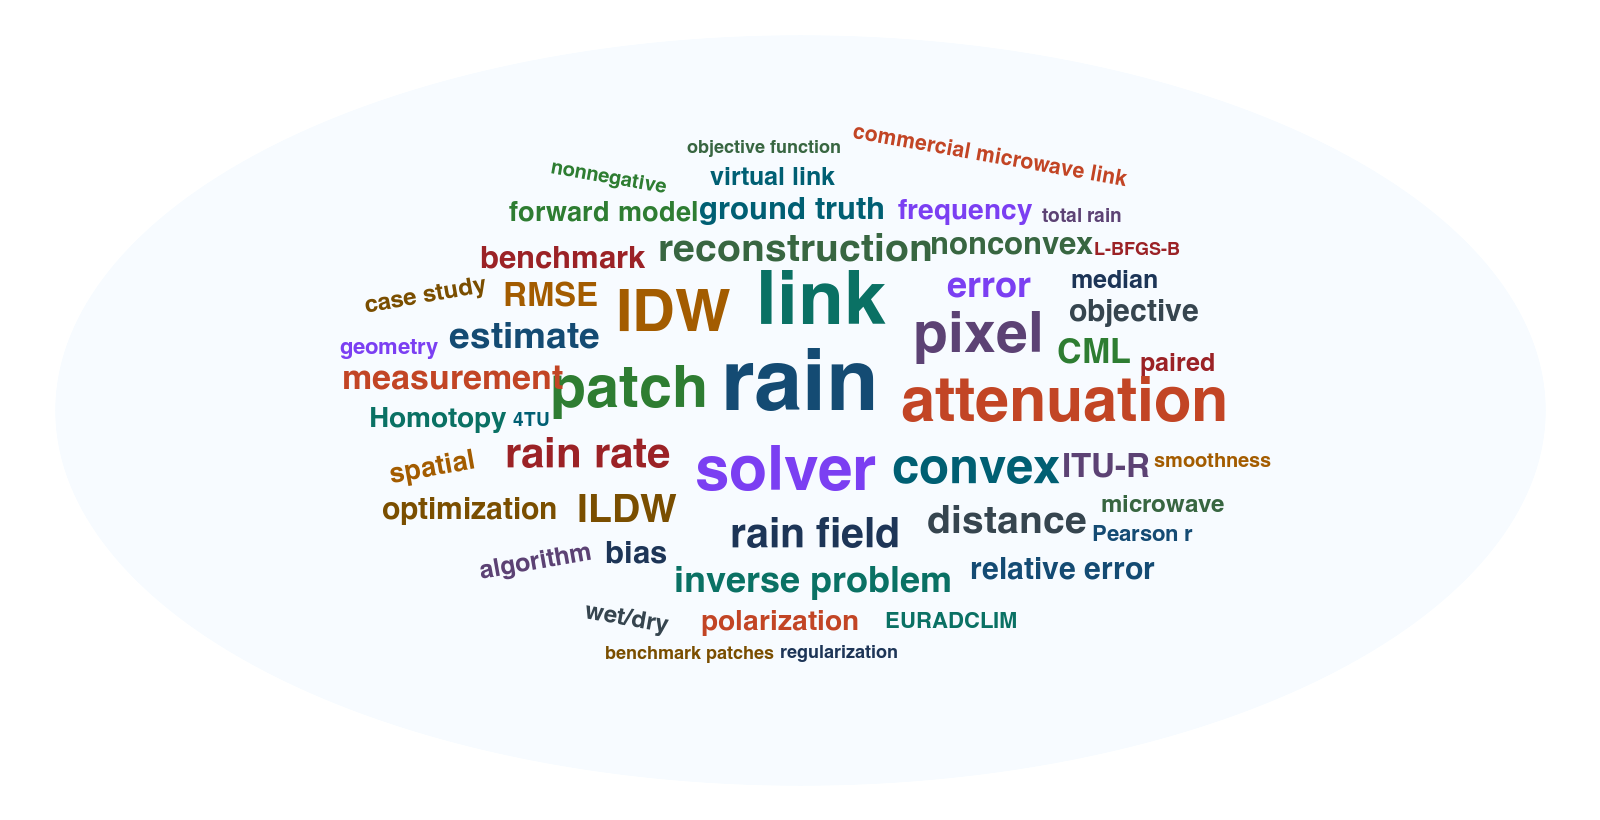
\includegraphics[width=0.98\textwidth,height=0.80\textheight,keepaspectratio]{word-cloud.png}
\end{frame}

%%%%%%%%%%%%%%%%%%%%%%%%%%%%%%%%%%%%%%%%%%%%%%%%%%

\begin{frame}[plain]
    \vspace{-0.5mm}
    \begin{center}\large\bfseries Glossary: Microwave Links\end{center}
    \vspace{4mm}

    \textbf{Commercial microwave link (CML).}

    \vspace{1mm}
    A wireless connection between two antennas. Such links are used in 5G backhaul networks. In this talk, a link is represented by a line segment $\ell$.

    \vspace{3mm}
    \textbf{Frequency.}

    \vspace{1mm}
    The carrier frequency of the microwave signal.

    \vspace{3mm}
    \textbf{Polarization.}

    \vspace{1mm}
    The orientation of the electric field of the microwave signal.
\end{frame}



%%%%%%%%%%%%%%%%%%%%%%%%%%%%%%%%%%%%%%%%%%%%%%%%%%

\begin{frame}[plain]
    \vspace{-0.5mm}
    \begin{center}\large\bfseries Glossary: Rain Field and Attenuation\end{center}
    \vspace{4mm}

    \vspace{3mm}
    \textbf{Rain field.}

    \vspace{1mm}
    A function from a rectangular geographic area $\Omega$ to non-negative real values:
    \[
        R:\Omega \to \mathbb{R}_{\ge 0}.
    \]
    For a pixel $s\in\Omega$, $R(s)$ is the rain rate at that pixel, measured in mm/h.

    \vspace{3mm}
    \textbf{Attenuation.}

    \vspace{1mm}
    Water molecules are electric dipoles, so raindrops interact with the microwave signal, as in a microwave oven. This weakens the signal and reduces the received signal power.
\end{frame}

%%%%%%%%%%%%%%%%%%%%%%%%%%%%%%%%%%%%%%%%%%%%%%%%%%

\begin{frame}[plain]
    \vspace{-0.5mm}
    \begin{center}\large\bfseries Glossary: Forward Model\end{center}
    \vspace{4mm}

    \textbf{Forward model.}

    \vspace{1mm}
    A known function that maps the hidden object to the measurements:
    \[
        \text{object} \longrightarrow \text{measurements}.
    \]

    \vspace{3mm}
    \textbf{In our case.}

    \vspace{1mm}
    The hidden object is the rain field $R$, and the measurements are the link attenuations:
    \[
        R \longrightarrow \{A_\ell\}_\ell .
    \]

\end{frame}

%%%%%%%%%%%%%%%%%%%%%%%%%%%%%%%%%%%%%%%%%%%%%%%%%%

\begin{frame}[plain]
    \vspace{-0.5mm}
    \begin{center}\large\bfseries Glossary: Inverse Problem\end{center}
    \vspace{4mm}

    \textbf{Inverse problem.}

    \vspace{1mm}
    Recover the hidden object from the measurements:
    \[
        \text{measurements} \longrightarrow \text{estimated object}.
    \]

    \vspace{3mm}
    \textbf{In our case.}

    \vspace{1mm}
    Given the link attenuations, estimate the rain field:
    \[
        \{A_\ell\}_\ell \longrightarrow \hat R .
    \]

    \vspace{3mm}
    \textbf{Ground truth and reconstruction.}

    \vspace{1mm}
    The true rain field is denoted by $R$. An algorithm returns an estimated rain field $\hat R$.
\end{frame}
%%%%%%%%%%%%%%%%%%%%%%%%%%%%%%%%%%%%%%%%%%%%%%%%%%

\begin{frame}[plain]
    \vspace{-0.5mm}
    \begin{center}\large\bfseries Glossary: Evaluation Metrics\end{center}
    \vspace{3mm}

    Let $R_i$ be the ground-truth rain rate at pixel $i$, and let $\hat R_i$ be the estimated rain rate.

    \[
        \mathrm{Bias}
        =
        \frac{1}{n}\sum_{i=1}^n(\hat R_i-R_i) \quad \text{{\footnotesize the sample mean of the error $e_i=\hat R_i-R_i$.}}
    \]



    \[
        \mathrm{RMSE}
        =
        \sqrt{\frac{1}{n}\sum_{i=1}^n(\hat R_i-R_i)^2} \quad \text{{\footnotesize standard deviation of the error if the bias is zero}}
    \]




    \vspace{2mm}
    \textbf{Pearson correlation.}   covariance of the standardized variables = cosine of angle between $R$ and $\hat{R}$.
    \[
        r
        =
        \frac{\sum_i(\hat R_i-\bar{\hat R})(R_i-\bar R)}
        {\sqrt{\sum_i(\hat R_i-\bar{\hat R})^2}
            \sqrt{\sum_i(R_i-\bar R)^2}}
    \]

\end{frame}
%%%%%%%%%%%%%%%%%%%%%%%%%%%%%%%%%%%%%%%%%%%%%%%%%%

\begin{frame}[plain]
    \vspace{-0.5mm}
    \begin{center}\Large\bfseries append slide saying, now i can present my EGU slides. add a funny image with a relief from a pain\end{center}
    \vspace{3mm}

    \centering
    \begin{tikzpicture}[line width=0.8pt, font=\small]
        % Before glossary: terminology headache.
        \node[align=center] at (-4.2,2.1) {\textbf{Before glossary}};
        \draw[fill=orange!15] (-4.2,0.8) circle (0.55);
        \fill (-4.4,0.92) circle (0.04);
        \fill (-4.0,0.92) circle (0.04);
        \draw (-4.45,0.62) .. controls (-4.25,0.78) and (-4.15,0.78) .. (-3.95,0.62);
        \draw[red!70!black, line width=1pt] (-4.8,1.45) -- (-5.15,1.85) -- (-4.75,1.75) -- (-5.05,2.15);
        \draw[red!70!black, line width=1pt] (-3.6,1.45) -- (-3.25,1.85) -- (-3.65,1.75) -- (-3.35,2.15);
        \node[draw, rounded corners, fill=red!5, align=center, font=\scriptsize, text width=2.3cm]
        at (-4.2,-0.45) {CML? attenuation?\\RMSE? Pearson?};

        % Transition arrow.
        \draw[-{Latex[length=3mm]}, line width=1.0pt, blue!60!black]
        (-2.35,0.75) -- (1.35,0.75)
        node[midway, above, align=center, font=\scriptsize] {glossary\\pain relief};

        % After glossary: relaxed presenter.
        \node[align=center] at (3.4,2.1) {\textbf{After glossary}};
        \draw[fill=green!12] (3.4,0.8) circle (0.55);
        \fill (3.2,0.92) circle (0.04);
        \fill (3.6,0.92) circle (0.04);
        \draw (3.12,0.65) .. controls (3.28,0.45) and (3.52,0.45) .. (3.68,0.65);
        \node[draw, rounded corners, fill=blue!5, align=center, font=\scriptsize, text width=2.3cm]
        at (3.4,-0.45) {EGU slides\\ready to go};
        \draw[fill=white] (4.15,0.25) rectangle (5.0,1.25);
        \node[font=\scriptsize, align=center] at (4.575,0.75) {slides};
        \draw (3.85,0.45) -- (4.15,0.55);
        \node[font=\large] at (2.3,1.55) {Ahhh!};
    \end{tikzpicture}
\end{frame}
